\section{Die Eulersche Zahl auf 1.000.000 Stellen}
bevor ich die Eulersche Zahl auf eine Million stellen berechnen wollte, hatte ich sie mithilfe eines Python-moduls für arbiträre Präzision bereits auf einhunderttausend Stellen berechnet. Seitdem hatte mir ein Familienangehöriger über den Tröpfelalgorithmus erzählt, mit dem man die Eulersche Zahl von alleine arbiträre Präzision berechnen kann.
\subsection{Der Tröpfelalgorithmus}
der Tröpfelalgorithmus funktioniert so:
\begin{table}[h]
\centering
\begin{tabular}{|l|llllll|}
\hline
\rowcolor[HTML]{CBCEFB} 
{\color[HTML]{000000} } & {\color[HTML]{000000} 2} & {\color[HTML]{000000} 3} & {\color[HTML]{000000} 4} & {\color[HTML]{000000} 5} & {\color[HTML]{000000} 6} & {\color[HTML]{000000} 7} \\ \hline
2                       & 1                        & 1                        & 1                        & 1                        & 1                        & 1                        \\
\rowcolor[HTML]{DAE8FC} 
7                       & 0                        & 1                        & 0                        & 1                        & 5                        & 3                        \\
1                       & 1                        & 1                        & 3                        & 4                        & 0                        & 1                        \\
\rowcolor[HTML]{DAE8FC} 
8                       & 0                        & 1                        & 2                        & 0                        & 2                        & 6                        \\ \hline
\end{tabular}
\caption{Kleine Tabelle zur Veranschaulichung / als Beispiel}
\end{table}
\par Erstelle eine Tabelle. Reihe 0 Besteht aus einer leeren Stelle am anfang und danach 2,3,4,... bis zu einer zahl n, sodass n! die so viele stellen hat wie man nachkomma stellen berechnen möchte. Reihe 1 beginnt mit einer 2 (welches bereits die Vorkommastelle von $e$ darstellt) und ist von nur 1 gefolgt. Um die Nächste reihe Zu berechnen beginne ganz Rechts in der jetzigen Spalte und multipliziere das Feld mit 10. Teile das durch das Feld darüber, schreibe den Rest in das Untere Feld und addiere den Übertrag zum Feld rechts, Nachdem du den wert dort ebenfalls mal 10 multipliziert hat (im falle man ist ganz Rechts angekommen, dann schreibt man den übertrag unten rechts in die Reihe der Nachkommastellen). wenn man Diesen Vorgang wiederholt, dann erscheinen die Ziffern von $e$ in basis 10 als die Erste Reihe der Tabelle.
\subsubsection{die Genauigkeit des Tröpfelalgorithmus}
\begin{figure}[h]
  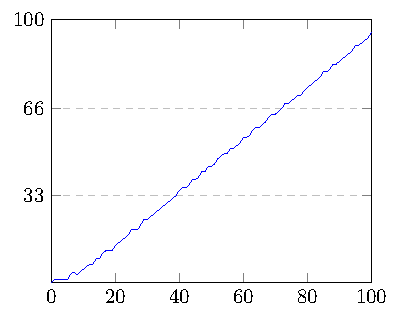
\includegraphics{medien2/1mil/1mil.pdf}
  \centering
  \caption{die Genauigkeit des Tröpfelalgorithmus}
\end{figure}
\par
von der Grafik könnte man erwarten, dass der Tröpfelalgorithmus sei langsamer als 
